\documentclass[10pt,a4paper]{article}
\usepackage[utf8]{inputenc}
\usepackage{polski}
\usepackage{amsmath}
\usepackage{amsfonts}
\usepackage{amssymb}
\usepackage{graphicx}
\usepackage{verbatim}
\usepackage{minted}

\author{Onaszkiewicz Przemysław, Gadawski Łukasz}
\title{Rozwiązanie zadania komiwojażera przy pomocy algorytmu genetycznego. - wersja sekwencyjna działająca na pojedynczym procesorze.}

\begin{document}
\maketitle

\section{Cel zadania}
Celem pierwszego etapu projektu jest implementacja wersji sekwencyjnej algorytmu genetycznego działającego na pojedynczym procesorze do rozwiązywania problemu komiwojażera.

\section{Problem komiwojażera}
Problem zdefiniowany jest następująco: mając listę miast oraz odległości między nimi, znajdź najkrótszą, dozwoloną drogę (początkiem oraz końcem drogi jest ten sam wierzchołek), zawierającą każde miasto dokładnie raz. Inaczej problem polega na znalezieniu minimalnego cyklu Hamiltona w pełnym grafie ważonym. Problem należy do zbioru problemów NP-trudnych.

\section{Algorytm genetyczny}
W 1975 roku przez Johna Hollanda został wynaleziony algorytm genetyczny, którego zadaniem było działanie analogiczne do procesu ewolucji na ziemi. Pseudokod prostego algorytmu genetycznego (ang. \textit{Simple Genetic Algorithm}) został przedstawiony poniżej:
\begin{minted}{bash}
procedure "Simple Genetic Algorithm"
begin 
	t := 0
	initilize P^{t}
	evaluate P^{t}
	while (not stop_condition)
	begin
		O^{t} = reproduce P^{t}
		crossover O^{t}
		mutate O^{t}
		evaluate O^{t}
		P^{t + 1} := O^{t}
		t := t + 1
	end
end
\end{minted}

$sum - $

\section{Implementacja}

\subsection{Tworzenie mapy miast}
W naszej implementacji mapa została odwzorowana jako obiekt posiadający wielkość, zbiór miast oraz strukturę danych \textit{mapa} gdzie kluczem jest para miasto-miasto oraz odległość między taką na mapie.

\subsubsection{Wczytanie z pliku}
Mapę odległości między miastami można odczytać z pliku tekstowego o strukturze przedstawionej poniżej. W pierwszej linii pliku znajdują się wierzchołki grafu oddzielone tabulatorami. W kolejnych liniach znajdują się krawędzie grafu(po jednej krawędzi na linię) w postacie wierzchołek - wierzchołek - wartość. Separatorem w pliku jest tabulator. Przykład pliku przedstawiono poniżej.

\begin{minted}{bash}
0	1	2	3
0	1	100
0	2	10
0	3	10
1	2	20
1	3	70
2	3	50
\end{minted}{bash}
\subsubsection{Losowa generacja mapy}

Możliwa jest losowa generacja mapy poprzez wywołanie metody :
\begin{minted}{bash}
shared_ptr<Map> Map::ConstructMapOfSize(int mapSize,
		int lowestPossibleDistance = 0, int highestPossibleDistance = 200)
\end{minted}
Podana metoda konstruuje mapę miast o zadanej wielkości, która jest grafem pełnym. Krawędzie grafu które są odległościami między miastami mają losowe wartości pomiędzy wartościami zadanymi w parametrach  \textit{lowestPossibleDistance i highestPossibleDistance}. 

\subsection{Konfiguracja programu}
Konfiguracja programu jest możliwa przy pomocy pliku \textit{app.properties}. Umożliwia on zdefiniowanie następujących parametrów:
\begin{itemize}
\item[--] \textbf{population\_size} - wielkość populacji w każdej iteracji algorytmu,
\item[--] \textbf{propability\_of\_crossover} - prawdopodobieństwo krzyżowania,
\item[--] \textbf{propability\_of\_mutation} - prawdopodobieństwo mutacji,
\item[--] \textbf{generation\_number} - liczba pokoleń, czyli iteracji algorytmu, w przypadku naszej implementacji jest to warunek stopu.
\end{itemize}

Przykładowa zawartość pliku konfiguracyjnego została zamieszczona poniżej.
\begin{minted}{bash}
population_size=5
propability_of_crossover=0.20
propability_of_mutation=0.01
generation_number=3
\end{minted}
\section{Testy}
Przeprowadzono testy z działania programu. Dzielą się one na dwie części. Pierwszą z nich jest Sprawdzenie poprawności algorytmu na niewielkich grafach. Kolejną jest przetestowanie efektywności zrównoleglenia algorytmu.
\subsection{Testy poprawności}
Jako dane wejściowe sprawdzające poprawność działania algorytmu wykorzystano dwa, małe, tendencyjnie stworzone grafy, w których można z łatwością dokonać weryfikacji działania algorytmu.Schematy podanych grafów przedstawiono poniżej.

\begin{figure}[H]
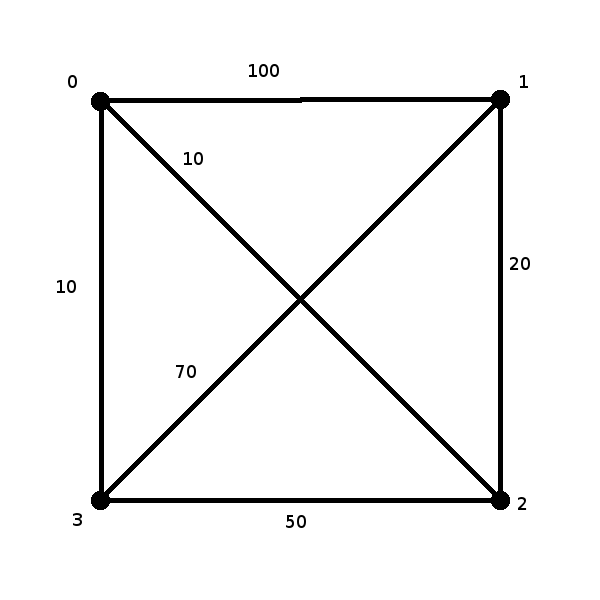
\includegraphics[scale=0.5]{mapa4.png}
\centering
\caption{\label{graph4}Graf wejściowy zawierający 4 wierzchołki}
\end{figure}
Po przetworzeniu pliku wejściowego zawierającego graf \ref{graph4} Algorytm wyznaczył najkrótszą ścieżkę o wartości 110. Należy pamiętać że ostatnim odcinkiem pokonywanym przez kuriera jest droga z ostatniego odwiedzonego miasta do miasta z którego wyruszył. W tym przypadku jest to krawędź pomiędzy wierzchołkami 1 i 3 o wartości 70. Najważniejsze fragmenty pliku wejściowego zostały przedstawione poniżej. 

\begin{minted}{bash}
POPULATION SIZE: 30

map size: 4
nodes:0 1 2 3 
m[first city: 0 sec city: 1] = 100
m[first city: 0 sec city: 2] = 10
m[first city: 0 sec city: 3] = 10
m[first city: 1 sec city: 2] = 20
m[first city: 1 sec city: 3] = 70
m[first city: 2 sec city: 3] = 50


Initial population initialization time: 7154 microseconds

START reproduce

START reproduce
0 'st generation production time: 22464 microseconds

START reproduce
1 'st generation production time: 14053 microseconds

START reproduce
2 'st generation production time: 9021 microseconds

START reproduce
3 'st generation production time: 362 microseconds

START reproduce
4 'st generation production time: 339 microseconds

START reproduce
5 'st generation production time: 357 microseconds

whole loop time 46596

 END: 3->0->2->1

PAth LEN: 110
\end{minted}{bash}

\begin{figure}[H]
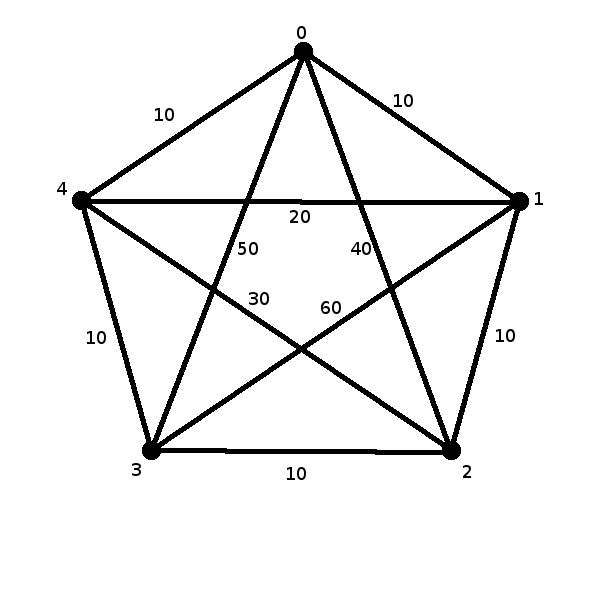
\includegraphics[scale=0.5]{mapa5.png}
\centering
\caption{\label{graph5}Graf wejściowy zawierający 5 wierzchołków}
\end{figure}

Po przetworzeniu pliku z grafem wejściowym przedstawionego na rysunku \ref{graph5} program wyznaczył ścieżkę o wartości 50. Najważniejsze fragmenty pliku wejściowego zostały przedstawione poniżej.

\begin{minted}{bash}
map size: 5
nodes:0 1 2 3 4 
m[first city: 0 sec city: 1] = 10
m[first city: 0 sec city: 2] = 40
m[first city: 0 sec city: 3] = 50
m[first city: 0 sec city: 4] = 10
m[first city: 1 sec city: 2] = 10
m[first city: 1 sec city: 3] = 60
m[first city: 1 sec city: 4] = 20
m[first city: 2 sec city: 3] = 10
m[first city: 2 sec city: 4] = 30
m[first city: 3 sec city: 4] = 10


Initial population initialization time: 8892 microseconds

START reproduce

START reproduce
0 'st generation production time: 14998 microseconds

START reproduce
1 'st generation production time: 14012 microseconds

START reproduce 
2 'st generation production time: 14433 microseconds

START reproduce
3 'st generation production time: 11731 microseconds

START reproduce 
4 'st generation production time: 12254 microseconds

START reproduce
5 'st generation production time: 18946 microseconds

whole loop time 86374

END: 4->0->1->2->3

PAth LEN: 50
\end{minted}{bash}

\subsection{Testy efektywności zrównoleglenia}
Kolejnym etapem testów było przetestowanie efektywności zrównoleglenia kodu. Wykorzystanie poszczególnych rdzeni procesora zostało przedstawione na rysunkach poniżej. Jeden z nich przedstawia wykonanie szeregowe programu, drugi zaś wykonanie zrównoleglone.


\begin{figure}[H]
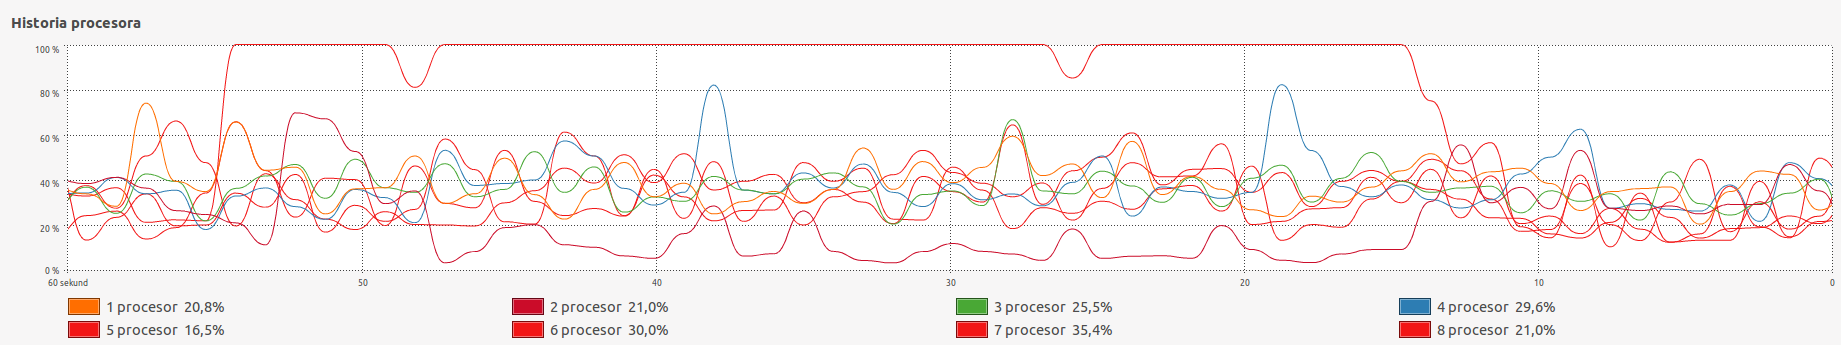
\includegraphics[scale=0.2]{zrzutSequence.png}
\centering
\caption{\label{diagramSequence}Diagram przedstawiający zużycie wątków przy wykonaniu sekwencyjnym}
\end{figure}

\begin{figure}[H]
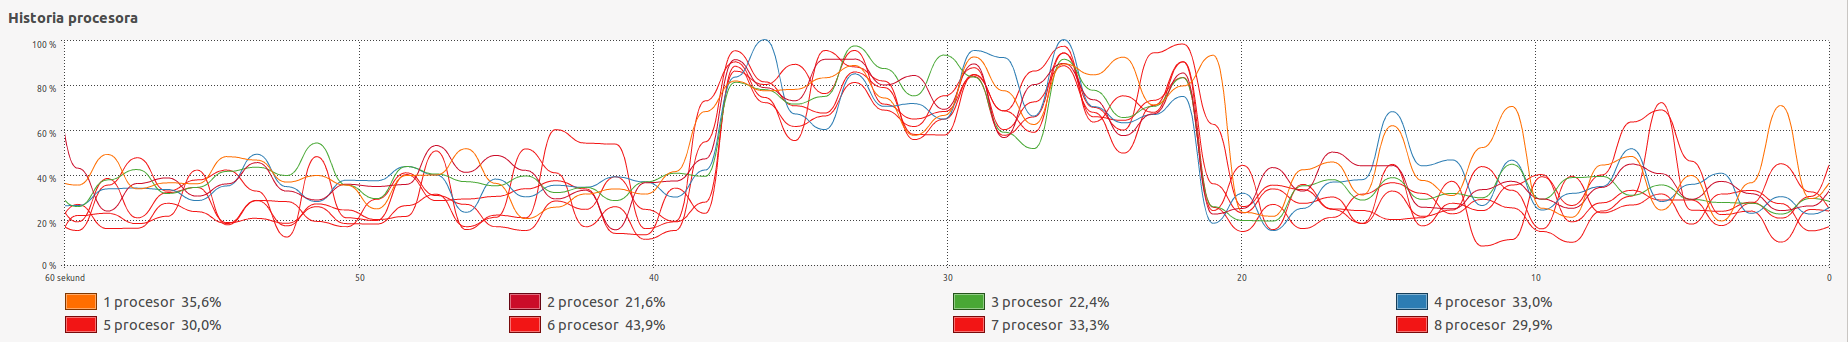
\includegraphics[scale=0.2]{zrzutParallel.png}
\centering
\caption{\label{diagramParallel}Diagram przedstawiający zużycie wątków przy wykonaniu zrównoleglonym}
\end{figure}


Zrównoleglenie algorytmu za pomozą dyrektyw OpenMP powoduje około trzykrotne zmniejszenie czasu wykonania programu. Pliki wynikowe outSequence.txt i outParallel.txt przedstawiają Wyjście algorytmu w formie sekwencyjnej i zrównoleglonej Ze względu na ich długość poniżej zostały przedstawione niewielnie, lecz najważniejsze wycinki.

\begin{minted}{bash}
Parallel: whole_time = 40832015 microseconds
Sequential: whole_time = 16281865 microseconds
\end{minted}{bash}

Następują niewielkie wahania współczynnika przyspieszenia, ale generalnie utrzymuje się on na poziomie około 3 (trzyktortne przyspieszenie po użyciu dyrektyw OpenMP)

\section{Wnioski}

\section{Podsumowanie}

\end{document}
